%%%%%%%%%%%%%%%%%%%%%%%%%%%%%%%%%%%%%%%%%
% Programming/Coding Assignment
% LaTeX Template
%
% This template has been downloaded from:
% http://www.latextemplates.com
%
% Original author:
% Ted Pavlic (http://www.tedpavlic.com)
%
% Note:
% The \lipsum[#] commands throughout this template generate dummy text
% to fill the template out. These commands should all be removed when 
% writing assignment content.
%
% This template uses a Perl script as an example snippet of code, most other
% languages are also usable. Configure them in the "CODE INCLUSION 
% CONFIGURATION" section.
%
%%%%%%%%%%%%%%%%%%%%%%%%%%%%%%%%%%%%%%%%%

%----------------------------------------------------------------------------------------
%	PACKAGES AND OTHER DOCUMENT CONFIGURATIONS
%----------------------------------------------------------------------------------------

\documentclass{article}

\usepackage{fancyhdr} % Required for custom headers
\usepackage{lastpage} % Required to determine the last page for the footer
\usepackage{extramarks} % Required for headers and footers
\usepackage[usenames,dvipsnames]{color} % Required for custom colors
\usepackage{graphicx} % Required to insert images
\usepackage{listings} % Required for insertion of code
\usepackage{courier} % Required for the courier font
\usepackage{lipsum} % Used for inserting dummy 'Lorem ipsum' text into the template
\usepackage[utf8]{inputenc}
\usepackage[ngerman]{babel}
\usepackage{minted}

% Margins
\topmargin=-0.45in
\evensidemargin=0in
\oddsidemargin=0in
\textwidth=6.5in
\textheight=9.0in
\headsep=0.25in

\linespread{1.1} % Line spacing

% Set up the header and footer
\pagestyle{fancy}
%\lhead{\hmwkAuthorName} % Top left header
\chead{\hmwkClass\ : \hmwkTitle} % Top center head
\rhead{\firstxmark} % Top right header
\lfoot{\lastxmark} % Bottom left footer
\cfoot{} % Bottom center footer
\rfoot{Page\ \thepage\ of\ \protect\pageref{LastPage}} % Bottom right footer
\renewcommand\headrulewidth{0.4pt} % Size of the header rule
\renewcommand\footrulewidth{0.4pt} % Size of the footer rule

\setlength\parindent{0pt} % Removes all indentation from paragraphs

%----------------------------------------------------------------------------------------
%	CODE INCLUSION CONFIGURATION
%----------------------------------------------------------------------------------------

\definecolor{MyDarkGreen}{rgb}{0.0,0.4,0.0} % This is the color used for comments
\lstloadlanguages{Perl} % Load Perl syntax for listings, for a list of other languages supported see: ftp://ftp.tex.ac.uk/tex-archive/macros/latex/contrib/listings/listings.pdf
\lstset{language=Perl, % Use Perl in this example
        frame=single, % Single frame around code
        basicstyle=\small\ttfamily, % Use small true type font
        keywordstyle=[1]\color{Blue}\bf, % Perl functions bold and blue
        keywordstyle=[2]\color{Purple}, % Perl function arguments purple
        keywordstyle=[3]\color{Blue}\underbar, % Custom functions underlined and blue
        identifierstyle=, % Nothing special about identifiers                                         
        commentstyle=\usefont{T1}{pcr}{m}{sl}\color{MyDarkGreen}\small, % Comments small dark green courier font
        stringstyle=\color{Purple}, % Strings are purple
        showstringspaces=false, % Don't put marks in string spaces
        tabsize=5, % 5 spaces per tab
        %
        % Put standard Perl functions not included in the default language here
        morekeywords={rand},
        %
        % Put Perl function parameters here
        morekeywords=[2]{on, off, interp},
        %
        % Put user defined functions here
        morekeywords=[3]{test},
       	%
        morecomment=[l][\color{Blue}]{...}, % Line continuation (...) like blue comment
        numbers=left, % Line numbers on left
        firstnumber=1, % Line numbers start with line 1
        numberstyle=\tiny\color{Blue}, % Line numbers are blue and small
        stepnumber=5 % Line numbers go in steps of 5
}

% Creates a new command to include a perl script, the first parameter is the filename of the script (without .pl), the second parameter is the caption
\newcommand{\perlscript}[2]{
\begin{itemize}
\item[]\lstinputlisting[caption=#2,label=#1]{#1.pl}
\end{itemize}
}

%----------------------------------------------------------------------------------------
%	DOCUMENT STRUCTURE COMMANDS
%	Skip this unless you know what you're doing
%----------------------------------------------------------------------------------------

% Header and footer for when a page split occurs within a problem environment
\newcommand{\enterProblemHeader}[1]{
%\nobreak\extramarks{#1}{#1 continued on next page\ldots}\nobreak
%\nobreak\extramarks{#1 (continued)}{#1 continued on next page\ldots}\nobreak
}

% Header and footer for when a page split occurs between problem environments
\newcommand{\exitProblemHeader}[1]{
%\nobreak\extramarks{#1 (continued)}{#1 continued on next page\ldots}\nobreak
%\nobreak\extramarks{#1}{}\nobreak
}

\setcounter{secnumdepth}{0} % Removes default section numbers
\newcounter{homeworkProblemCounter} % Creates a counter to keep track of the number of problems

\newcommand{\homeworkProblemName}{}
\newenvironment{homeworkProblem}[1][Problem \arabic{homeworkProblemCounter}]{ % Makes a new environment called homeworkProblem which takes 1 argument (custom name) but the default is "Problem #"
\stepcounter{homeworkProblemCounter} % Increase counter for number of problems
\renewcommand{\homeworkProblemName}{#1} % Assign \homeworkProblemName the name of the problem
\section{\homeworkProblemName} % Make a section in the document with the custom problem count
\enterProblemHeader{\homeworkProblemName} % Header and footer within the environment
}{
\exitProblemHeader{\homeworkProblemName} % Header and footer after the environment
}

\newcommand{\problemAnswer}[1]{ % Defines the problem answer command with the content as the only argument
\noindent\framebox[\columnwidth][c]{\begin{minipage}{0.98\columnwidth}#1\end{minipage}} % Makes the box around the problem answer and puts the content inside
}

\newcommand{\homeworkSectionName}{}
\newenvironment{homeworkSection}[1]{ % New environment for sections within homework problems, takes 1 argument - the name of the section
\renewcommand{\homeworkSectionName}{#1} % Assign \homeworkSectionName to the name of the section from the environment argument
\subsection{\homeworkSectionName} % Make a subsection with the custom name of the subsection
\enterProblemHeader{\homeworkProblemName\ [\homeworkSectionName]} % Header and footer within the environment
}{
\enterProblemHeader{\homeworkProblemName} % Header and footer after the environment
}

%----------------------------------------------------------------------------------------
%	NAME AND CLASS SECTION
%----------------------------------------------------------------------------------------

\newcommand{\hmwkTitle}{Übung\ \#4} % Assignment title
\newcommand{\hmwkDueDate}{Dienstag,\ 18.\ November\ 2014} % Due date
\newcommand{\hmwkClass}{Reconfigurable Embedded Systems} % Course/class
\newcommand{\hmwkClassTime}{} % Class/lecture time
\newcommand{\hmwkClassInstructor}{} % Teacher/lecturer
\newcommand{\hmwkAuthorName}{Günther Schindler, Sven Dorkenwald, Kilian Bender} % Your name

%----------------------------------------------------------------------------------------
%	TITLE PAGE
%----------------------------------------------------------------------------------------

\title{
\vspace{2in}
\textmd{\textbf{\hmwkClass:\ \hmwkTitle}}\\
\normalsize\vspace{0.1in}\small{Abgabe\ am\ \hmwkDueDate}\\
\vspace{0.1in}\large{\textit{\hmwkClassTime}}
\vspace{3in}
}

\author{\textbf{\hmwkAuthorName}}
\date{} % Insert date here if you want it to appear below your name

%----------------------------------------------------------------------------------------

\begin{document}

\maketitle

%----------------------------------------------------------------------------------------
%	TABLE OF CONTENTS
%----------------------------------------------------------------------------------------

%\setcounter{tocdepth}{1} % Uncomment this line if you don't want subsections listed in the ToC

\newpage
\tableofcontents
\newpage
%----------------------------------------------------------------------------------------
%	Intro
%----------------------------------------------------------------------------------------
\begin{homeworkProblem}[Intro]
Für die vierte Übung ist eine Schaltung zu realisieren, die einen Testpattern aus einem
128 Byte ROM liest, diesen über einen FIFO mit zwei unterschiedlichen Takten schiebt und 
je vier Bit an den Datenausgang leitet. Für den getakteten Ausgang ist das, zum Lesen aus 
dem FIFO verwendete, Taktsignal an den Ausgang zu routen.
\begin{center}
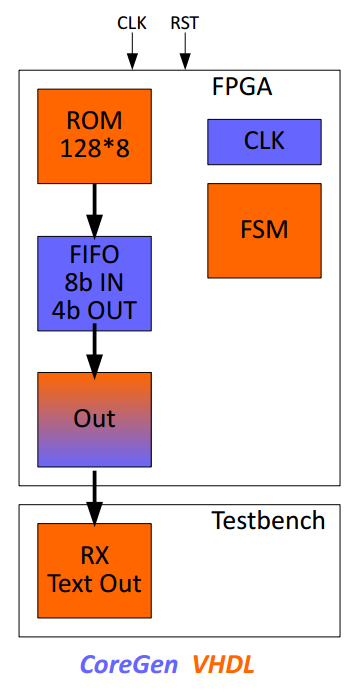
\includegraphics[width=0.3\columnwidth]{image}
\end{center}
\end{homeworkProblem}
%----------------------------------------------------------------------------------------
%	ROM
%----------------------------------------------------------------------------------------
\begin{homeworkProblem}[ROM]
Das ROM von 128 Byte soll über VHDL-Code beschrieben werden. Dazu wird der subtype word\_t
eingeführt welcher ein Byte umfasst. Der Typ memory\_t ist ein Array aus 128 word\_t und 
wird für das ROM verwendet. Um Schreibarbeit zu sparen, wurde die Funktion init\_rom 
implementiert. Diese Funktion initialisiert das ROM mit den Werten 1-128.
\begin{minted}{vhdl}
architecture Behavioral of exercise4 is
...
  subtype word_t is std_logic_vector(7 downto 0);
  type memory_t is array(127 downto 0) of word_t;

  function init_rom
    return memory_t is
      variable tmp : memory_t := (others => (others => '0'));
      variable count_value : integer := 1;
        begin
          for addr_pos in 0 to 127 loop
          tmp(addr_pos) := std_logic_vector(to_unsigned(count_value,8));
          count_value := count_value + 1;
      end loop;
    return tmp;
  end init_rom;
  
  constant rom : memory_t := init_rom;
  ...
end Behavioral;
\end{minted}

\end{homeworkProblem}

%----------------------------------------------------------------------------------------
%	Clock
%----------------------------------------------------------------------------------------

\begin{homeworkProblem}[Clock]
Mithilfe des Core-Generators sind die Taktfrequenzen 100 MHz und 200 MHz zu realisieren.
Dazu werden vom Core-Generator erstellte Komponente (clk) in den VHDL-Code eingebunden.
Der Takteingang der Komponente (CLK\_IN1) wird mit dem Entity-Eingang (clk\_in) und somit
mit dem internen 100 MHz des Atlys-Board verbunden. Die beiden Taktausgänge (CLK\_OUT1 und 
CLK\_OUT2) liefern die benötigten 100 und 200 MHz.
\begin{minted}{vhdl}
architecture Behavioral of exercise4 is
  ...
  component clk
  port
   (-- Clock in ports
    CLK_IN1           : in     std_logic;
    -- Clock out ports
    CLK_OUT1          : out    std_logic;
    CLK_OUT2          : out    std_logic;
    -- Status and control signals
    RESET             : in     std_logic);
  end component;
  ...
  begin
  ...
  clk_instance : clk
  port map
  (-- Clock in ports
    CLK_IN1 => clk_in,
    -- Clock out ports
    CLK_OUT1 => clk_1,
    CLK_OUT2 => clk_2,
    -- Status and control signals
    RESET  => reset_in
  );
  ...
end Behavioral;
\end{minted}
\end{homeworkProblem}

%----------------------------------------------------------------------------------------
%	FIFO
%----------------------------------------------------------------------------------------

\begin{homeworkProblem}[FIFO]
Als nächstes ist ein FIFO zu realisieren. Es soll mit den zwei unterschiedlichen 
Taktsignalen (clk\_1=100MHz, clk\_2=200MHz) betrieben werden und unterschiedliche Schreibe-
und Lesebreite (8- und 4-Bit) haben. Das FIFO soll mit minimaler Schreibtiefe (16-Bit) und 
als First-Word-Fall-Thru betrieben werden. Das FIFO soll über den CoreGen realisiert werden.
\\
Diese beschriebenen Eigenschaften lassen sich einfach über die grafische oberfläche des
Core-Generators einstellen. Danach kann die Komponente in den VHDL-Code eingebunden werden.
Der Port wr\_clk wird mit den 100 MHz und der Port rd\_clk mit den 200 MHz verbunden.
Die 8-Bit Daten werden über einen Register (wreg) aus dem ROM gelesen (rom(addr)) und mit
dem Dateneingang des FIFO (din) verbunden. Der Datenausgang (dout) wird über einen Register
(rreg) mit dem Entity-Ausgang dout verbunden.
\begin{minted}{vhdl}
architecture Behavioral of exercise4 is
  ...
  COMPONENT fifo
  PORT (
    rst : IN STD_LOGIC;
    wr_clk : IN STD_LOGIC;
    rd_clk : IN STD_LOGIC;
    din : IN STD_LOGIC_VECTOR(7 DOWNTO 0);
    wr_en : IN STD_LOGIC;
    rd_en : IN STD_LOGIC;
    dout : OUT STD_LOGIC_VECTOR(3 DOWNTO 0);
    full : OUT STD_LOGIC;
    empty : OUT STD_LOGIC
  );
  END COMPONENT;
  ..
  begin
  ...
  fifo_instance : fifo
  PORT MAP (
    rst => reset_in,
    wr_clk => clk_1,
    rd_clk => clk_2,
    din => din,
    wr_en => wr_en,
    rd_en => rd_en,
    dout => dout_int,
    full => full,
    empty => empty
  );
  ...
  -- write register
  wreg : process(clk_1)
  begin
    if(rising_edge(clk_1)) then
      din <= rom(addr);
    end if;
  end process;
  -- read register
  rreg : process(clk_2)
  begin
    not_clk_2 <= not clk_2;
    if(rising_edge(clk_2)) then
      dout <= dout_int;
    end if;
  end process;
  ...
end Behavioral;
\end{minted}
\end{homeworkProblem}

%----------------------------------------------------------------------------------------
%	Finite State Machine
%----------------------------------------------------------------------------------------

\begin{homeworkProblem}[Finite State Machine]
Die Finite State Machines übernehmen die Schreibe- und Lese-Kontrolle der Schaltung. Es
wurde eine FSM für die Lesekontrolle und eine FSM für die Schreibekontrolle realisiert.
Die FSMs haben je 2 States (IDLE, RDWT). Über die zwei State Register (sreg\_1 und sreg\_2)
werden die beiden FSMs an die Schreibfrequenz (100MHz) und Lesefrequenz (200MHz) gebunden.
\\
In den FSMs wird überprüft ob der FIFO voll (full) oder leer (empty) ist und dem entsprechend
wird das Schreiben in den FIFO (wr\_en) bzw. das Lesen aus dem FIFO (rd\_en) ermöglicht oder
gesperrt. 
\begin{minted}{vhdl}
architecture Behavioral of exercise4 is
  ...
  -- signals for FSM
  type fsm_t is (IDLE,  RDWT);
  signal cstate_1, nstate_1 : fsm_t;
  signal cstate_2, nstate_2 : fsm_t;
  ..
  begin
  ...
  -- state register 1
  sreg_1 : process
  begin
    wait until rising_edge(clk_1);
    if reset_in = '1' then
      cstate_1 <= IDLE;
    else
      cstate_1 <= nstate_1;
    end if;
  end process;
  -- state register 2
  sreg_2 : process
  begin
    wait until rising_edge(clk_2);
    if reset_in = '1' then
      cstate_2 <= IDLE;
    else
      cstate_2 <= nstate_2;
    end if;
  end process;
  --state logic
  sproc_1 : process(clk_1, cstate_1, full)
  begin
    nstate_1 <= cstate_1;
    wr_en <= '0';
    case cstate_1 is
    when IDLE =>
      if(full = '0') then
        nstate_1 <= RDWT;
        wr_en <= '1';
      else
        nstate_1 <= IDLE;
        wr_en <= '0';
      end if;
    when RDWT =>
      if(full = '0') then
        nstate_1 <= RDWT;
        wr_en <= '1';
      else
        nstate_1 <= IDLE;
        wr_en <= '0';
      end if;
    when others =>
      nstate_1 <= IDLE;
    end case;
  end process;
  
  --state logic
  sproc_2 : process(clk_2, cstate_2, empty)
  begin
    nstate_2 <= cstate_2;
    rd_en <= '0';
    case cstate_2 is
    when IDLE =>
      if(empty = '0') then
        nstate_2 <= RDWT;
        rd_en <= '1';
      else
        nstate_2 <= IDLE;
        rd_en <= '0';
      end if;
    when RDWT =>
      if(empty = '0') then
        nstate_2 <= RDWT;
        rd_en <= '1';
      else
        nstate_2 <= IDLE;
        rd_en <= '0';
      end if;
    when others =>
      nstate_2 <= IDLE;
    end case;
  end process;
  ...
end Behavioral;
\end{minted}
Die Adressen, für das Lesen des ROM, werden über den Prozess cproc gesteuert. Dieser Prozess
inkrementiert in Schreibegeschwindigkeit (100 MHz) die Adresse, sofern die FSM das Schreiben
in das FIFO ermöglicht hat (wr\_en = '1'). Erreicht die Adresse den Endwert (127) wird
wieder vom Anfang angefangen.
\begin{minted}{vhdl}
architecture Behavioral of exercise4 is
  ..
  begin
  ...
  cproc : process
  begin
    wait until rising_edge(clk_1);
    if(reset_in = '1') then
      addr <= 0;
    else
      if(addr < 127 and wr_en = '1') then
        addr <= addr + 1;
      elsif(addr=127 and wr_en = '1') then
        addr <= 0;
      end if;
    end if;
  end process;
  ...
end Behavioral;
\end{minted}
\end{homeworkProblem}
%----------------------------------------------------------------------------------------
%	Clocked Output
%----------------------------------------------------------------------------------------

\begin{homeworkProblem}[Clocked Output]
Basierend auf den Funktionalitäten des SelectIO Wizards soll ein Clock-Forwarding der 200 MHz 
auf einen Ausgangspin realisiert werden.
\\
Hier werden je eine Instanz des ODDR2 und des OBUF benötigt. Die beiden Takteingänge des
ODDR2 werden mit den Taktsignalen clk\_2 und not\_clk\_2 verbunden. Der Ausgang des 
ODDR2 wird mit dem Eingang des OBUF verbunden. Dessen Ausgang wird direkt zum
Entity-Ausgang geführt.
\begin{minted}{vhdl}
architecture Behavioral of exercise4 is
  ..
  begin
  ...
  oddr2_clk_inst : ODDR2
  generic map (
    DDR_ALIGNMENT  => "C0",
    INIT           => '0',
    SRTYPE         => "ASYNC")
  port map
    (D0             => '1',
    D1             => '0',
    C0             => not_clk_2,
    C1             => clk_2,
    CE             => '1',
    Q              => clk_fwd_out,
    R              => reset_in,
    S              => '0'
    );
    
  obuf_clk_inst : OBUF
  generic map (
    IOSTANDARD => "LVCMOS33")
  port map (
    O          => clk_out,
    I          => clk_fwd_out
    );
  ...
end Behavioral;
\end{minted}
\end{homeworkProblem}
%----------------------------------------------------------------------------------------
%----------------------------------------------------------------------------------------
%	Testbench
%----------------------------------------------------------------------------------------
\begin{homeworkProblem}[Testbench]
Die Testbench verundet in dem Prozess out\_proc je zwei 4-Bit Ausgangswerte und gibt diese
auf die Standardausgabe aus. Dadurch kann die korrekte Funktion der Schaltung bestätigt 
werden.

\begin{minted}{vhdl}
out_proc: process(dout)
  variable logline : line;
  begin
    doutput <= doutput(3 downto 0) & dout;
    if(flag = '1') then
      write(logline, doutput);
      writeline(output, logline);
    end if;
   flag <= not flag;
   end process;
-- Output
-- 00000001
-- 00000010
-- 00000011
-- ...
\end{minted}
\end{homeworkProblem}
%----------------------------------------------------------------------------------------
%	Summary
%----------------------------------------------------------------------------------------
\begin{homeworkProblem}[Summary]
Betrachtet man den Synthesereport sieht man, dass das 128 Byte Read Only RAM erkannt wurde.
Merkwürdig ist an dieser stelle, dass die FSM und der FIFO trotz korrekter Implementierung
nicht erkannt wurden.
\\\\
    $Found 8-bit register for signal <din>.
    \\Found 4-bit register for signal <dout>.
    \\Found 7-bit register for signal <addr>.
    \\Found 7-bit adder for signal
    \\Found 128x8-bit Read Only RAM for signal 
    \\Found 7-bit comparator greater for signal
    \\Summary:
    \\inferred   1 RAM(s).
    \\inferred   1 Adder/Subtractor(s).
    \\inferred  19 D-type flip-flop(s).
    \\inferred   1 Comparator(s).
    \\inferred   1 Multiplexer(s)$
\\\\
Aus dem Place and Route Report kann man folgende Werte entnehmen. Wobei die beiden 
8-Bit Ram vermutlich für das FIFO verwendet wurde (tiefe 2-Byte).
\\\\
$Number of Slice Registers   88
\\Number of Slice LUTs        53
\\Number of RAMB8BWERs         2
\\Number of used BUFGs         2$
\end{homeworkProblem}
\clearpage
%----------------------------------------------------------------------------------------
\end{document}